% This version of CVPR template is provided by Ming-Ming Cheng.
% Please leave an issue if you found a bug:
% https://github.com/MCG-NKU/CVPR_Template.

%\documentclass[review]{cvpr}
\documentclass[final]{cvpr}

\usepackage{times}
\usepackage{epsfig}
\usepackage{graphicx}
\usepackage{amsmath}
\usepackage{amssymb}

\usepackage{url}            % simple URL typesetting
\usepackage{booktabs}       % professional-quality tables
\usepackage{amsfonts}       % blackboard math symbols
\usepackage{nicefrac}       % compact symbols for 1/2, etc.
\usepackage{microtype}      % microtypography

\usepackage{graphicx}
\usepackage{amsmath,amssymb} % define this before the line numbering.
\usepackage{bbold}
\usepackage{dsfont}
\usepackage{enumerate}
\usepackage[toc,page]{appendix}
\usepackage[font=small,labelfont=bf]{caption}

\usepackage{enumitem}

\usepackage{xcolor}
\usepackage{caption}
% \usepackage{subcaption}
\usepackage{bm}
\usepackage{isomath}
\usepackage{arydshln}
\usepackage{stmaryrd}

% \usepackage{fixltx2e}
\usepackage{dblfloatfix}
\usepackage{pbox}
\usepackage{capt-of}

\usepackage[normalem]{ulem}
\usepackage{multirow}

\usepackage{colortbl}

\usepackage{mathtools}
\usepackage{array}

\makeatletter
\@namedef{ver@everyshi.sty}{}
\makeatother
\usepackage{pgf}

\newcommand{\xpt}{\edef\f@size{\@xpt}\rm}

\def\ie{\emph{i.e.}}
\def\etc{\emph{etc}}

\usepackage{tikz}

\newcommand{\comment}[1]{}

\usepackage{indentfirst}
% variables
%\vec{\mathcal{M}}
\renewcommand\vec[1]{\ensuremath\boldsymbol{#1}}
\renewcommand\cdots{...}
\newcommand{\tC}{\vec{\mathcal{C}}}
\newcommand{\tH}{\vec{\mathcal{H}}}
\newcommand{\tB}{\vec{\mathcal{B}}}
\newcommand{\tY}{\vec{\mathcal{Y}}}
\newcommand{\tF}{\vec{\mathcal{F}}}
\newcommand{\cB}{\mathcal{B}}
\newcommand{\mB}{\mathbf{B}}
\newcommand{\mY}{\mathbf{Y}}
\newcommand{\mZ}{\mathbf{Z}}
\newcommand{\vb}{\mathbf{b}}
\newcommand{\vy}{\mathbf{y}}
\newcommand{\valpha}{\bm{\alpha}}
\newcommand{\tX}{\vec{\mathcal{X}}}
\newcommand{\cX}{\mathcal{X}}
\newcommand{\mX}{\mathbf{X}}
\newcommand{\vx}{\mathbf{x}}
\newcommand{\mbrp}[1]{\mathbb{R}_{+}^{#1}}
\newcommand{\mbr}[1]{\mathbb{R}^{#1}}
\newcommand{\mbn}[1]{\mathbb{N}^{#1}}
\newcommand{\mbnz}[1]{\mathbb{N}_{0^+}^{#1}}
\newcommand{\mbnp}[1]{\mathbb{N}_{+}^{#1}}
\newcommand{\stackThree}{{;}_{3}}
\newcommand{\vbeta}{\vec{\beta}}
%\newcommand{\rank}[1]{\text{Rank}({#1})}

%\newcommand{\tXS}{\vec{\mathcal{X}}^{*}}
\newcommand{\vv}{\mathbf{v}}
\newcommand{\vq}{\mathbf{q}}
\newcommand{\tV}{\vec{\mathcal{V}}}
\newcommand{\tE}{\vec{\mathcal{E}}}
\newcommand{\tEH}{\vec{\mathcal{\hat{E}}}}
\newcommand{\tVH}{\vec{\mathcal{\bar{V}}}}
\newcommand{\tVT}{\vec{\mathcal{\hat{V}}}}
\newcommand{\idx}[1]{\mathcal{I}_{#1}}
\newcommand{\semipd}[1]{\mathcal{S}_{+}^{#1}}
\newcommand{\spd}[1]{\mathcal{S}_{++}^{#1}}

\newcommand{\tR}{\vec{\mathcal{R}}}
\newcommand{\vu}{\mathbf{u}}
\newcommand{\vup}{\mathbf{u^{'}}}
\newcommand{\vz}{\mathbf{z}}
\newcommand{\vzeta}{\boldsymbol{\zeta}}
\newcommand{\vc}{\mathbf{c}}

\newcommand{\vphi}{\boldsymbol{\phi}}
\newcommand{\vpsi}{\boldsymbol{\psi}}
\newcommand{\tPsi}{\vec{\mathcal{V}}}
\newcommand{\bigoh}{\mathcal{O}}
\newcommand{\mPsi}{\vec{\Psi}}
\newcommand{\vj}{\vec{j}}

% operators
\newcommand{\enorm}[1]{\left\|{#1}\right\|_2}
\newcommand{\fnorm}[1]{\left\|{#1}\right\|_F}
\newcommand{\lnorm}[1]{\left\|{#1}\right\|_1}
\newcommand{\riem}{\mathbf{d}_{\mathcal{R}}}
\newcommand{\spdp}[1]{\mathbb{S}_{++}^{#1}}
\newcommand{\simplex}[1]{\Delta^{#1}}
\newcommand{\set}[1]{\left\{#1\right\}}

\DeclareMathOperator*{\argmin}{arg\,min}
\DeclareMathOperator*{\argmax}{arg\,max}
\DeclareMathOperator*{\supp}{Supp}
\DeclareMathOperator*{\unique}{Unique}
\DeclareMathOperator*{\TRank}{TRank}
\DeclareMathOperator*{\rank}{Rank}
\DeclareMathOperator*{\spann}{Span}
\DeclareMathOperator*{\sym}{Sym}

\newcommand{\flatt}[1]{\text{Flatten}\!\left({#1}\right)}
\newcommand{\unflatt}[1]{\text{Flatten}^{-1}\!\left({#1}\right)}
\newcommand{\myspan}[1]{\spann\left(#1\right)}

\DeclareMathOperator*{\trace}{Tr}
%\DeclareMathOperator*{\rank}{Rank}
\DeclareMathOperator*{\kronstack}{\uparrow\!\otimes}

\DeclareMathOperator*{\avg}{avg}
\DeclareMathOperator*{\sgn}{Sgn}
\DeclareMathOperator*{\hosvd}{HOSVD}
\DeclareMathOperator*{\logm}{Log}
\DeclareMathOperator*{\detm}{Det}
\DeclareMathOperator*{\fg}{g}
\newcommand{\expl}[1]{\text{e}^{#1}}
\DeclareMathOperator*{\res}{Res}
\DeclareMathOperator*{\asinh}{Asinh}
%\newcommand{\exp}[1]{e^{#1}}




\newcommand{\mI}{\mathbf{I}}
\newcommand{\normvec}[1]{\frac{#1}{\|{#1}\|_2}}
\newcommand{\suptensor}[1]{\mathfrak{S}^{#1}}
\newcommand{\suptensorr}[2]{\mathfrak{S}^{#1}_{\times^{#2}}}
\newcommand{\region}{\mathcal{R}}

%\newtheorem{theorem}{Theorem}
%\newtheorem{definition}{Definition}
%\newtheorem{lemma}{Lemma}
%\newtheorem{proposition}{Proposition}
%\newtheorem{remark}{Remark}

\newcommand{\todo}[1]{{\bf \textcolor{red}{[TODO: #1]}}}


\newcommand{\mLa}{\bm{\lambda}^{*}}
\newcommand{\mLambda}{\bm{\lambda}}
\newcommand{\mU}{\bm{U}}
\newcommand{\mV}{\bm{V}}
\newcommand{\timetplone}{{(t+1)}}
\newcommand{\timet}{{(t)}}

\newcommand{\mBOvl}{{\mB^{*}}}

\newcommand{\piA}{{\Pi_A}}
\newcommand{\piB}{{\Pi_B}}

\newcommand{\sigmav}{{^v\!\!\,{\sigma}}}
%\newcommand{\thickhat}[1]{\mathbf{\ddot{\text{$#1$}}}}
\newcommand{\sigmas}{{^s\!\!\,{\sigma}}}

\newcommand{\fvx}{{\boldsymbol{f}(\vx)}}
\newcommand{\fvy}{{\boldsymbol{f}(\vy)}}

\newcommand{\vsss}{\boldsymbol{s}}
\newcommand{\vw}{\boldsymbol{w}}

\newcommand{\vphibar}{\boldsymbol{\bar{\phi}}}
\newcommand{\vsigma}{\boldsymbol{\sigma}}

\def\eg{\emph{e.g.}}

\newcommand{\myg}[1]{\boldsymbol{G}\left(#1\right)}
\newcommand{\mygtwo}[1]{\boldsymbol{G}\Big(#1\Big)}
%\newcommand{\mygthree}[1]{\boldsymbol{G}\left(#1\right)}
\newcommand{\mygthree}[1]{\boldsymbol{\mathcal{G}}\!\left(\!#1\!\right)}
\newcommand{\mygfour}[1]{\boldsymbol{\mathcal{G}}\!\Bigg(\!#1\!\Bigg)}
\newcommand{\tG}{\boldsymbol{\mathcal{G}}}

\newcommand{\vPhi}{\boldsymbol{\Phi}}
\newcommand{\invbeta}{{(1\!-\!\beta)}}
\newcommand{\invsqrtbeta}{\sqrt{1\!-\!\beta}}
\newcommand{\sqrtbeta}{\sqrt{\beta}}


\newcommand{\mIdent}{\boldsymbol{\mathds{I}}}
\newcommand{\sIdent}{\mathds{I}}
\newcommand{\vOnes}{\mathbb{1}}

\newcommand{\mJ}{\mathbf{J}}
\newcommand{\sXkl}{{X_{kl}}}

\newcommand{\mK}{\mathbf{K}}
\newcommand{\mKb}{\bar{\mK}}
\newcommand{\mKbb}{\bar{\mKb}}
\newcommand{\Kb}{\bar{K}}
\newcommand{\Kbb}{\bar{\Kb}}
\newcommand{\mC}{\mathbf{C}}

\newcommand{\mKro}{{\mK^{q}}}
\newcommand{\mKbro}{{\mKb{\,\!}^{q}}}
\newcommand{\mKbbro}{{\mKbb^{q}}}
\newcommand{\Kbro}{{\Kb^{q}}}
\newcommand{\Kbbro}{{\Kbb^{q}}}



\newcommand{\fvxt}{{\boldsymbol{f}^{(t)}(\vx)}}
\newcommand{\Fvxt}{{\boldsymbol{F}^{(t)}(\vx)}}
\newcommand{\fvxtplusone}{{\boldsymbol{f}^{(t+1)}(\vx)}}
\newcommand{\Fvxtplusone}{{\boldsymbol{F}^{(t+1)}(\vx)}}
\newcommand{\vxzero}{\mathbf{x}_0}
\newcommand{\fvxzerotplusone}{{\boldsymbol{f}^{(t+1)}(\vxzero)}}
\newcommand{\Fvxzerotplusone}{{\boldsymbol{F}^{(t+1)}(\vxzero)}}
\newcommand{\fvxzerotplusonei}{{\boldsymbol{f}_i^{(t+1)}(\vxzero)}}

\newcommand{\tFvxt}{{{\vec{\mathcal{F}}}^{(t)}(\vx)}}
\newcommand{\tFvxtplusone}{{{\vec{\mathcal{F}}}^{(t+1)}(\vx)}}
\newcommand{\tFvxzerotplusone}{{{\vec{\mathcal{F}}}^{(t+1)}(\vxzero)}}




\newcommand{\swbar}{\bar{w}}
\newcommand{\vwbar}{\bar{\boldsymbol{w}}}

\newcommand{\vvartheta}{\boldsymbol{\vartheta}}
\newcommand{\tprim}[1]{{\uparrow T_{#1}}}


\newcommand{\vS}{\boldsymbol{S}}

\newcommand{\barM}{{\bar{M}}}
\newcommand{\barmM}{{\bar{\vec{M}}}}

\newcommand{\sN}{\vec{N}}
\newcommand{\tN}{\vec{\mathcal{N}}}
\newcommand{\tP}{\vec{\mathcal{P}}}
\newcommand{\tS}{\vec{\mathcal{S}}}
\newcommand{\tSnb}{\mathcal{S}}
\newcommand{\mS}{\vec{S}}
\newcommand{\tNnb}{\mathcal{N}}

\newcommand{\cov}{\boldsymbol{\Sigma}}
\newcommand{\covb}{\boldsymbol{\Sigma}^{(\!\diamond\!)}}
\newcommand{\covw}{\boldsymbol{\Sigma}^{(\!*\!)}}
\newcommand{\vphix}[1]{{\boldsymbol{\phi}\left({#1}\right)}}
\newcommand{\covbb}[1]{{\boldsymbol{\Sigma}^{(\diamond,{#1})}}}
\newcommand{\covww}[1]{{\boldsymbol{\Sigma}_c^{(*,{#1})}}}

\newcommand{\muw}{\boldsymbol{\mu}^{(*)}}
\newcommand{\mub}{\boldsymbol{\mu}^{(\diamond)}}

\newcommand{\mubb}[1]{{\boldsymbol{\mu}^{(\diamond,{#1})}}}
\newcommand{\muww}[1]{{\boldsymbol{\mu}_c^{(*,{#1})}}}
\newcommand{\muwww}[2]{{\boldsymbol{\mu}_{#1}^{(*,{#2})}}}

\newcommand{\mPhi}{\boldsymbol{\Phi}}
\newcommand{\parsmP}{\!\left(\mPhi\right)}
\newcommand{\parsmPc}{\!\left(\mPhi_c\right)}
\newcommand{\parsmPA}{\!\left(\mPhi^A\right)}
\newcommand{\parsmPB}{\!\left(\mPhi^B\right)}
\newcommand{\parsmPAB}{\!\left(\mPhi^A\!,\mPhi^B\right)}
\newcommand{\parsmPcA}{\!\left(\mPhi_c^A\right)}
\newcommand{\parsmPcB}{\!\left(\mPhi_c^B\right)}
\newcommand{\parsmPxY}[2]{{\!\left(\mPhi_{#1}^{#2}\right)}}

\newcommand{\mMu}{\boldsymbol{M}}
\newcommand{\mM}{\boldsymbol{M}}
\newcommand{\parsmMu}{\!\left(\mMu\right)}
\newcommand{\mW}{\boldsymbol{W}}
\newcommand{\mD}{\boldsymbol{D}}
\newcommand{\mT}{\boldsymbol{T}}

\newcommand{\vmu}{\boldsymbol{\mu}}
\newcommand{\bvmu}{\boldsymbol{\overline{\mu}}}
\newcommand{\mP}{\boldsymbol{\Theta}}
\newcommand{\vmubar}{\boldsymbol{\bar{\mu}}}
\newcommand{\vvarphi}{\boldsymbol{\varphi}}


\newcommand{\stkout}[1]{{\ifmmode\text{\sout{\ensuremath{#1}}}\else\sout{#1}\fi}}

\newcommand{\mL}{\mathbf{L}}

\DeclareMathOperator*{\arcsinh}{arcsinh}

% Include other packages here, before hyperref.
\usepackage[numbib]{tocbibind}
% If you comment hyperref and then uncomment it, you should delete
% egpaper.aux before re-running latex.  (Or just hit 'q' on the first latex
% run, let it finish, and you should be clear).
\usepackage[pagebackref=true,breaklinks=true,colorlinks,bookmarks=false]{hyperref}


\def\cvprPaperID{8501} % *** Enter the CVPR Paper ID here
\def\confYear{CVPR 2021}
%\setcounter{page}{4321} % For final version only

\pagestyle{plain}
%\thispagestyle{empty}

\begin{document}

%%%%%%%%% TITLE
\title{Video Matting with Convolutional LSTM}
\author{\underline{Jiahao Zhang} \\ U6921098 \and Peng Zhang \\ U6921163 \and Hang Zhang \\ U6921112}

\maketitle
\begin{abstract}
    TODO
\end{abstract}

\section{Introduction}

\begin{figure}[htb]
    \centering
    \subfloat[Input video frames.]{
        \label{demo1}
        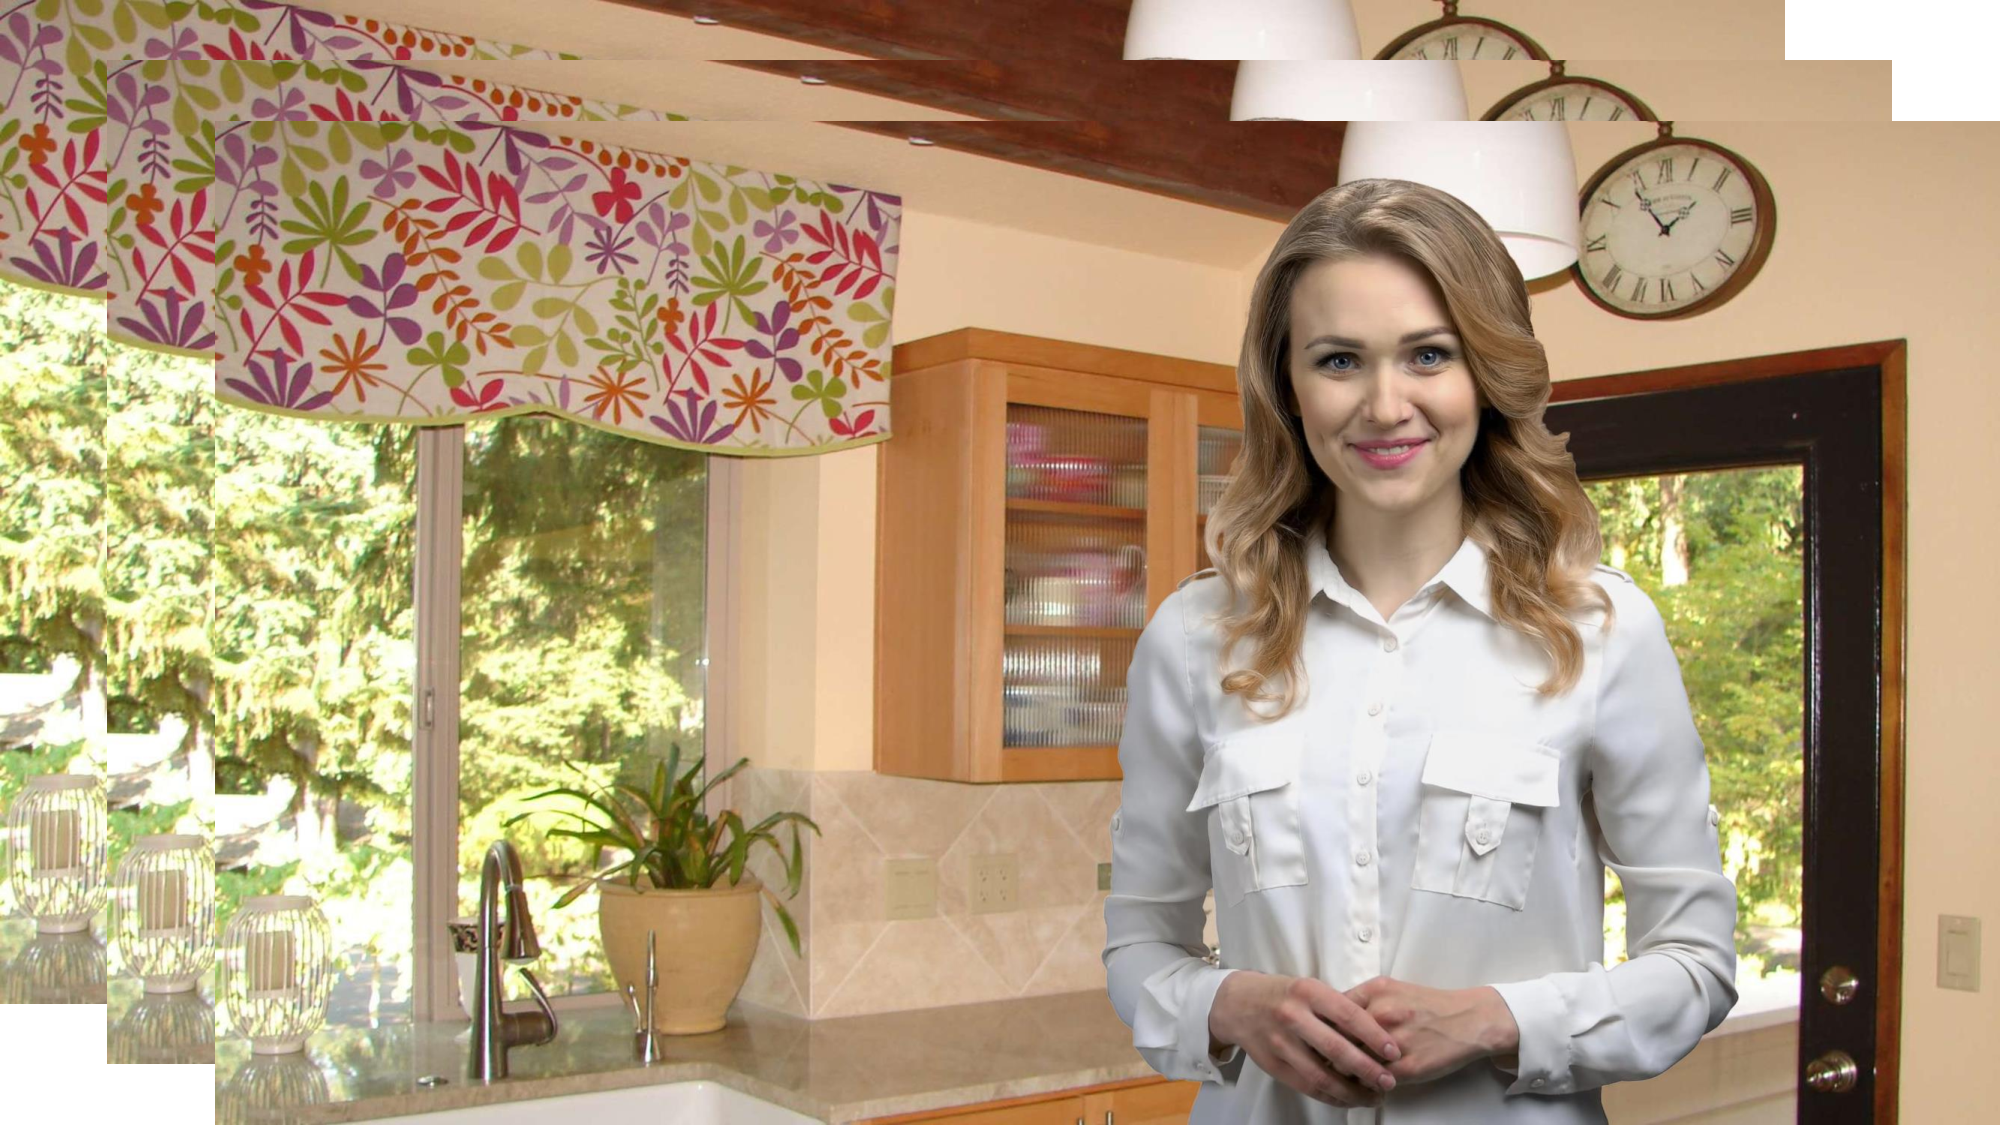
\includegraphics[width=0.47\linewidth]{img/demo1.pdf}
    }
    \subfloat[Output alpha mattes.]{
        \label{demo2}
        \includegraphics[width=0.47\linewidth]{img/demo2.pdf}
    }\\
    \subfloat[Background replacement.]{
        \label{demo3}
        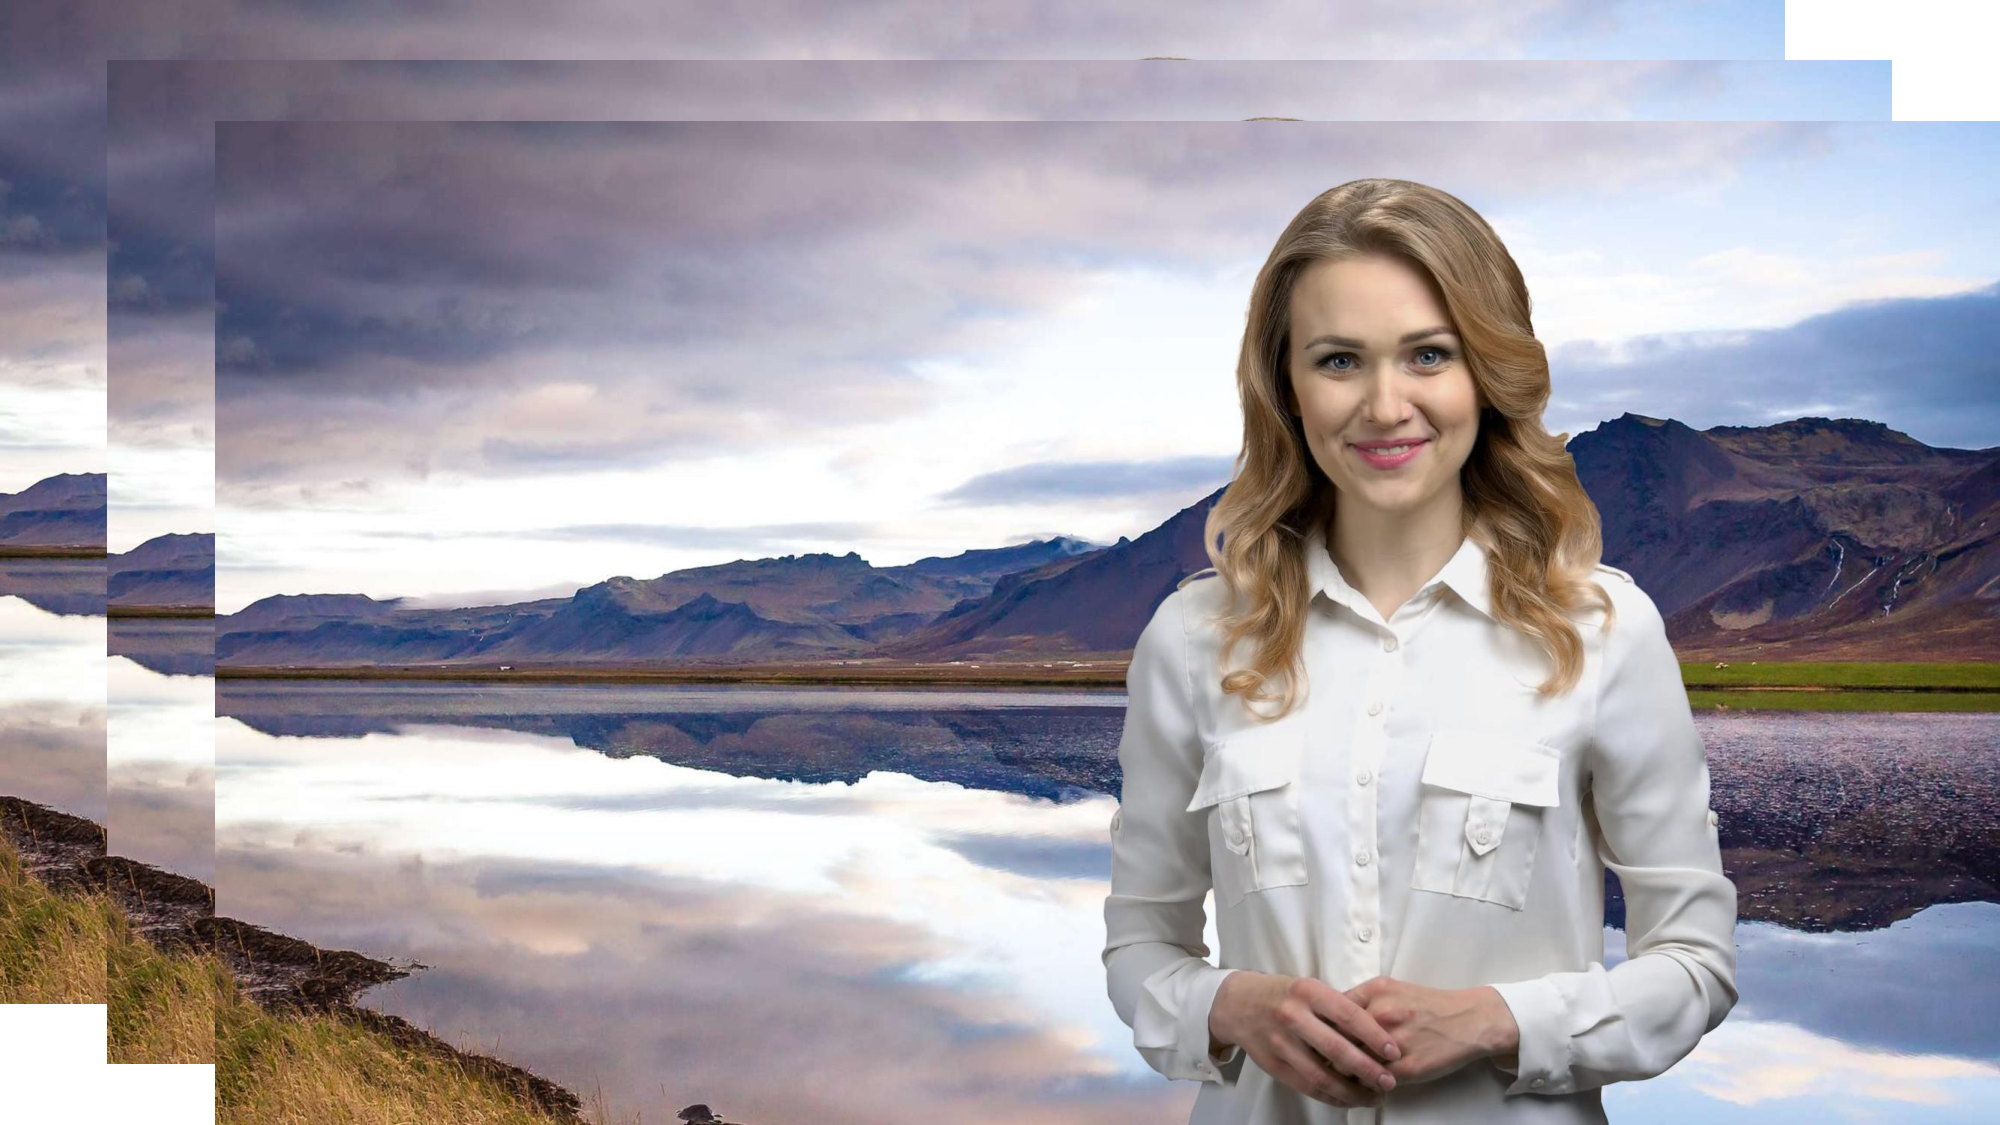
\includegraphics[width=0.47\linewidth]{img/demo3.pdf}
    }
    \subfloat[DanMu avoidance.]{
        \label{demo4}
        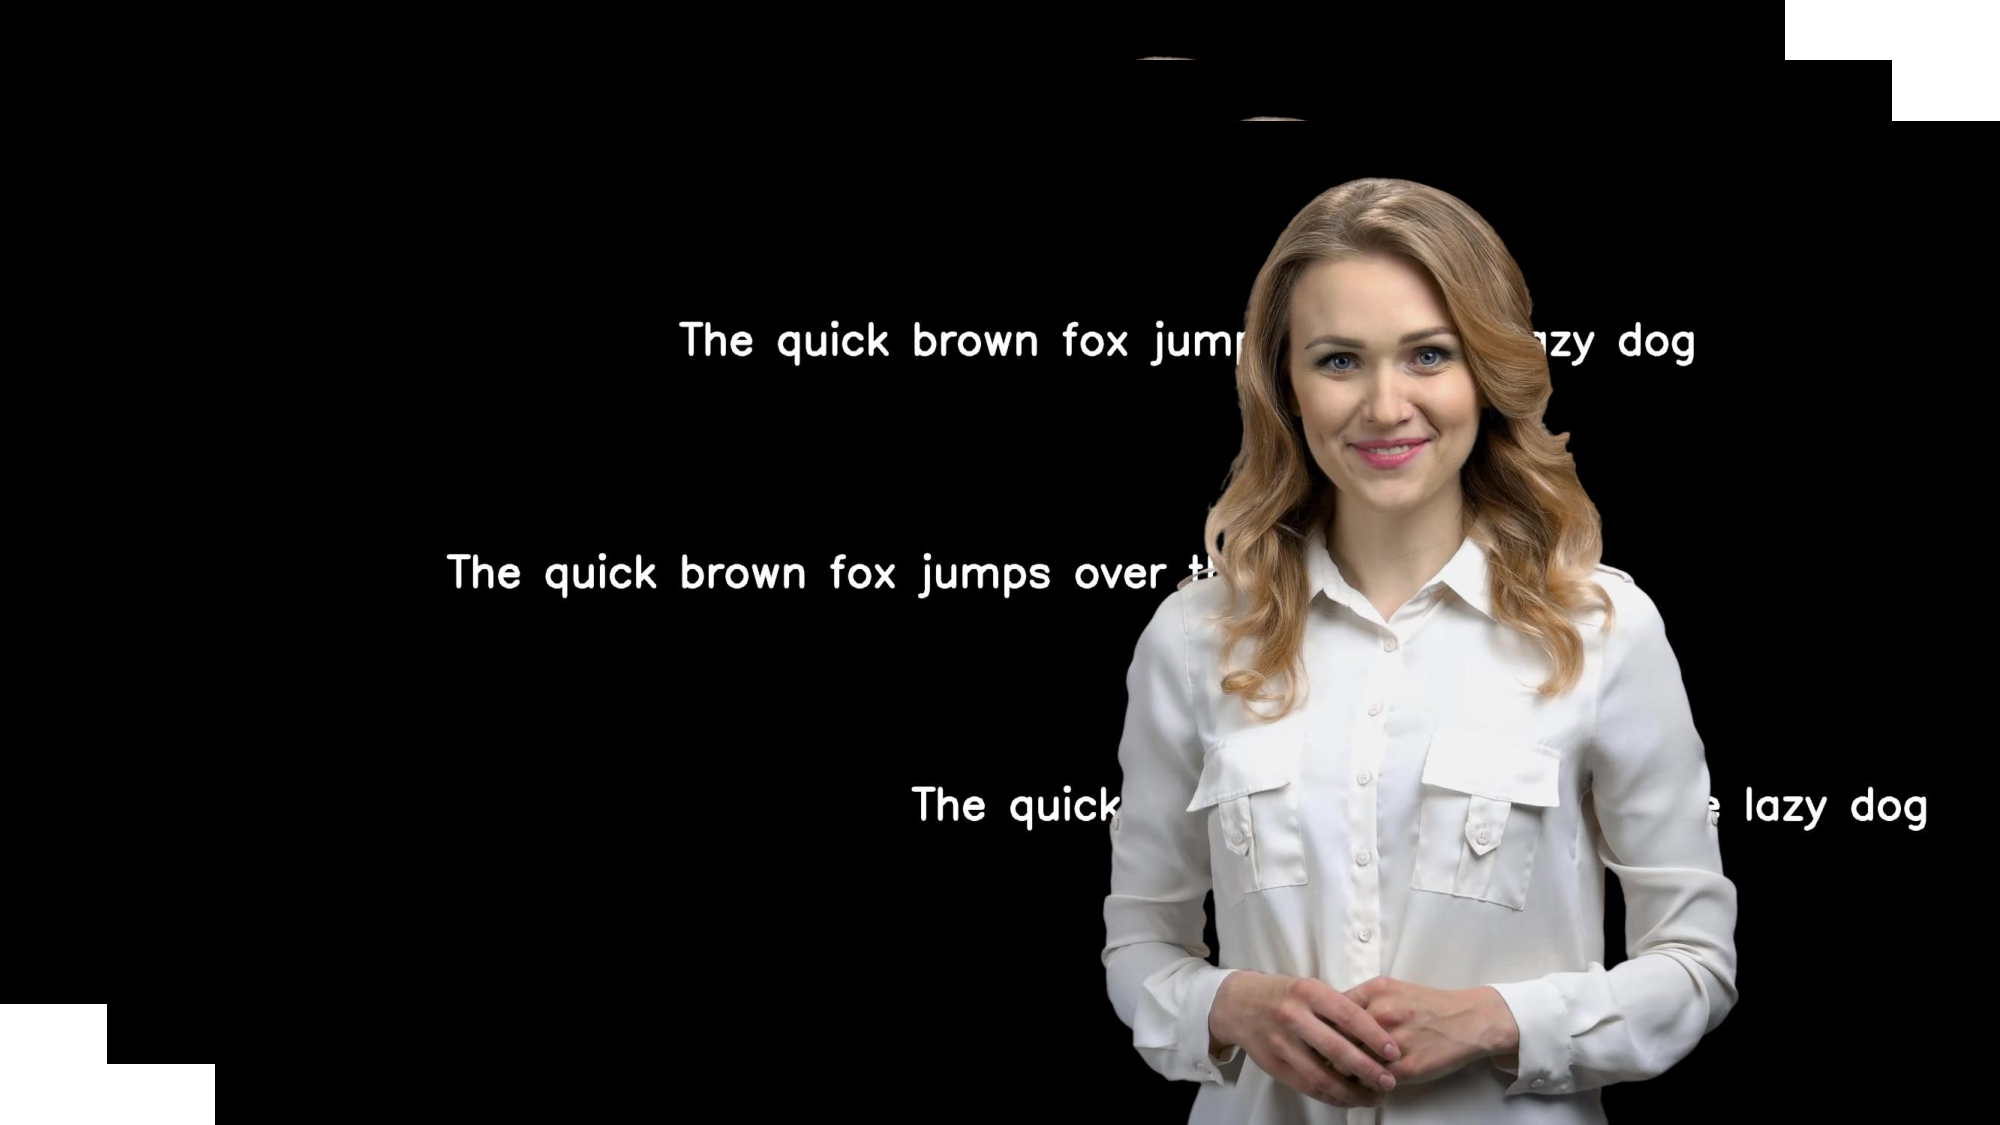
\includegraphics[width=0.47\linewidth]{img/demo4.pdf}
    }
    \caption{Demonstration of video matting.}
    \label{demo}
\end{figure}

\begin{figure*}[htb]
    \begin{center}
        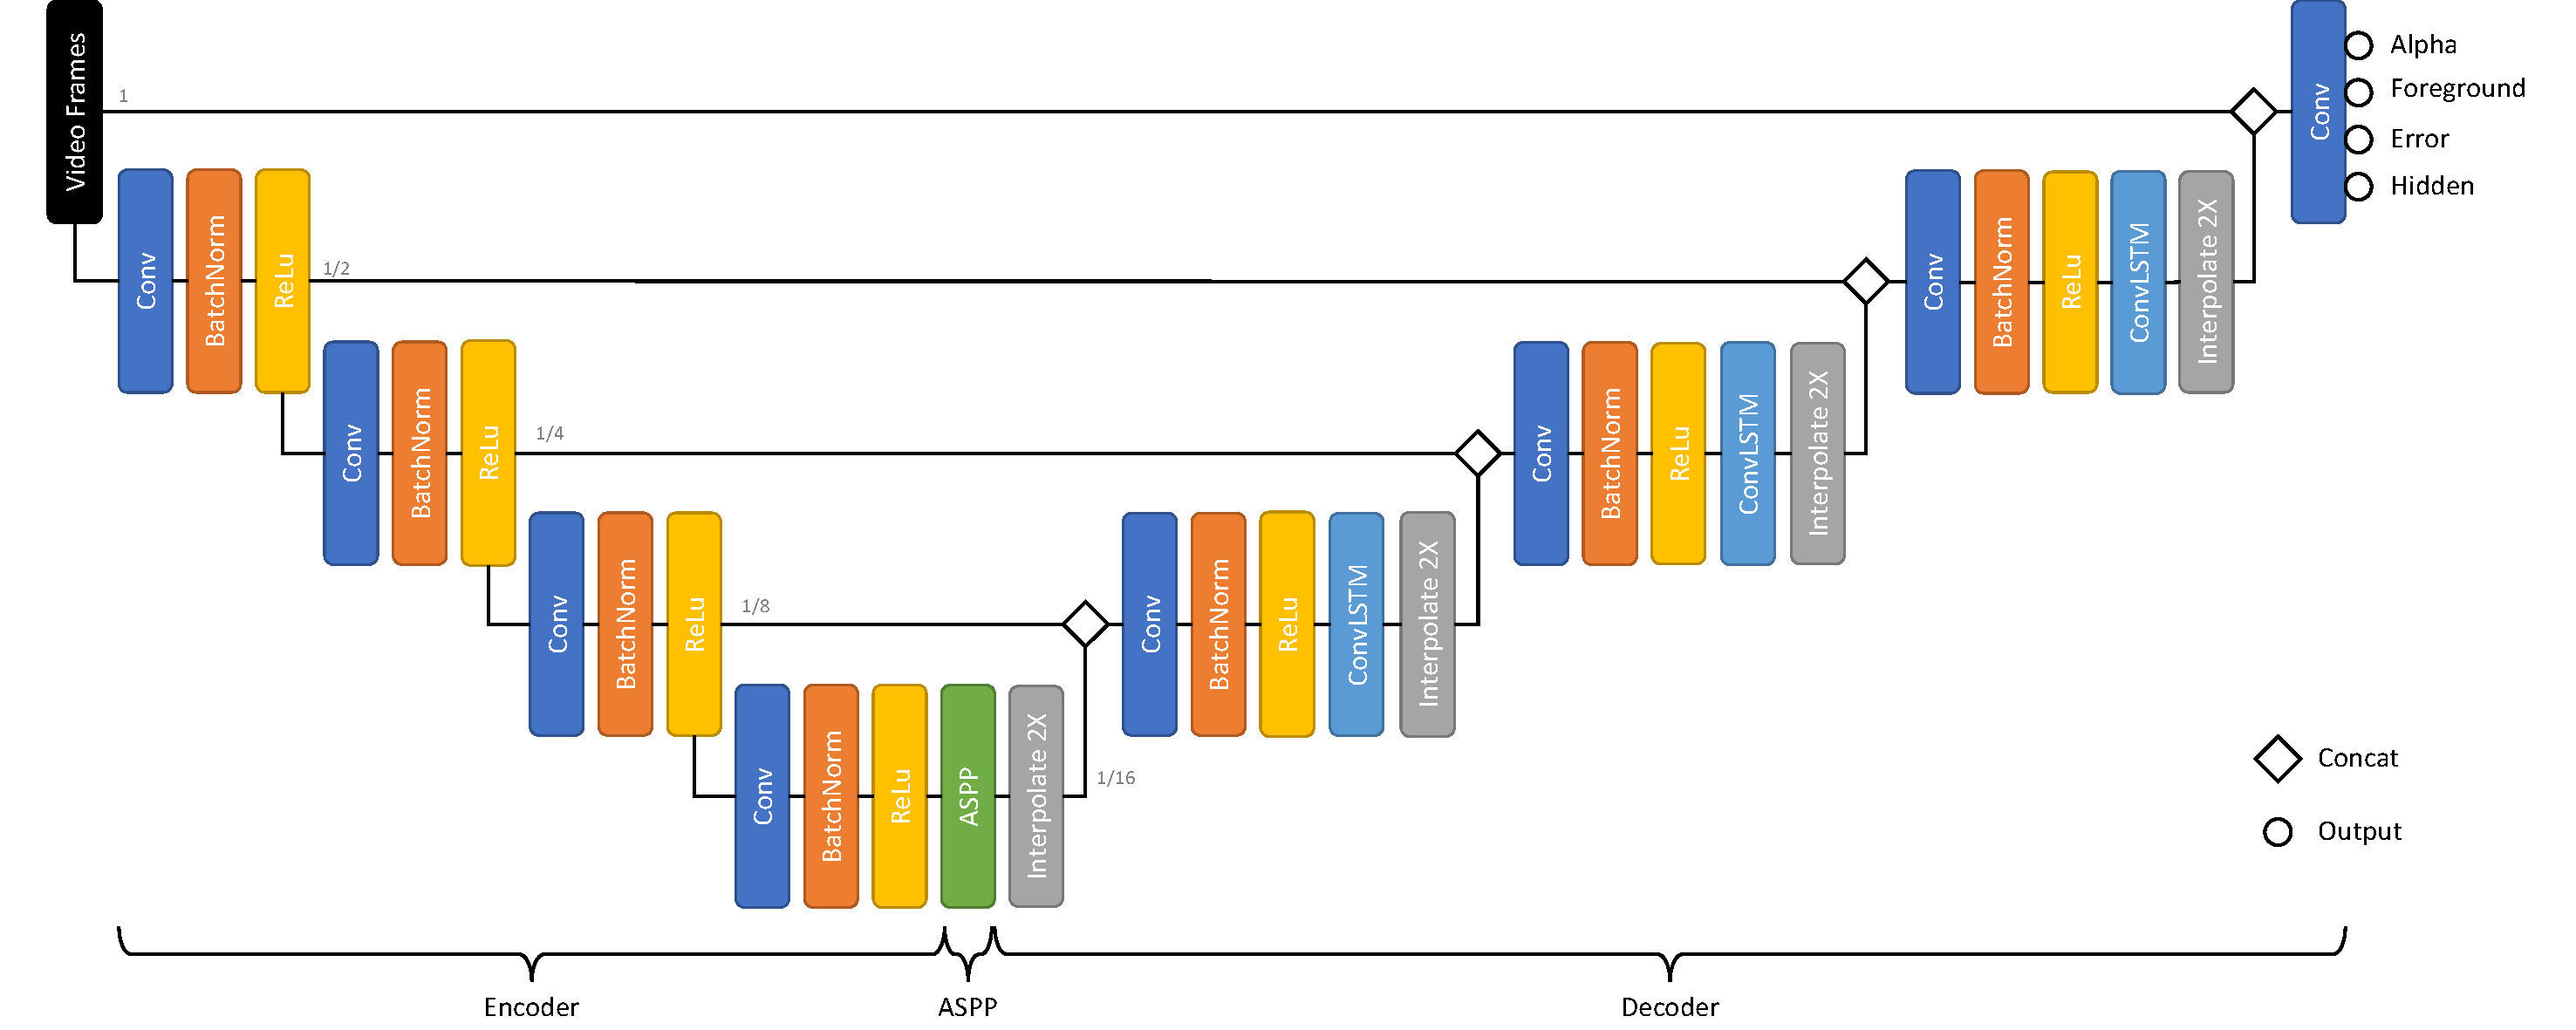
\includegraphics[width=1\textwidth]{img/modelConvLSTM.pdf}
    \end{center}
    \caption{The architecture of our model.}
    \label{modelConvLSTM}
\end{figure*}

With the global pandemic of Covid-19, online meetings via tools like Zoom and Microsoft Teams have become daily routine.
Background removal or replacement \ref{demo3} have become essential features to protect customers' privacy.
Besides that, DanMu or bullet chat has been grown with a large number of followers across different video websites like BiliBili and AcFun.
Despite its entertainment, DanMu avoidance \ref{demo4} has become a standard feature to reduce visual clutters and highlight the subject.
A key challenge is that users of online conference application are rare to possess a green screen like those designed for movie special effects and for better user experience, you cannot require them to do so. As for online videos, it hard to obtain alpha mattes after the video is made with traditional methods.

Lin et al. \cite{linRealTimeHighResolutionBackground2020a} proposed a method for a similar task, but it requires an extra background image as input.
Which is not suitable for the circumstances we mentioned above.
Plus, with the input background image, we can directly get the alpha matte by subtracting background from input image.
So we built up an end-to-end deep learning model to address this problem, which takes only video frames as input \ref{demo1} and outputs alpha mattes \ref{demo2} directly.
To alleviate the negative impact caused by removing background, we add convolutional recurrent neural network modules to enhance temporal information learning.
Combined with spatial features extracted from convolutional layers, we think the model should be able to learn and remember the previously displayed background, and motions of both background and foreground.

\paragraph{Semantic Segmentation}

Ever since U-Net \cite{Ronneberger2015UNetCN} proposed for biomedical image segmentation, Encoder-Decoder has become the standard architecture for semantic segmentation.
In the encoder, the size of feature maps gets smaller and the number of channels increases to gain larger and more informative receptive field.
The latent features are then passed to the decoder, where feature maps are scaled up to match the input size.
Skip connections between encoder and decoder provides the ability to pass information at different level of data compression.
DeepLab V2 \cite{Chen2018DeepLabSI} and V3 \cite{chenRethinkingAtrousConvolution2017} introduces Atrous Spatial Pyramid Pooling (ASPP), which uses Atrous convolution as pooling operator to enhance the ability for increasing receptive field wittout loosing information.
Because video image matting can be regarded as a binary semantic segmentation task initially, we adapt it as our base model.

\paragraph{Video Matting}

The method proposed by \cite{linRealTimeHighResolutionBackground2020a} contains a $G_{base}$ model based on DeepLab v3 and a Path-Refinement $G_{refine}$ model inspired by \cite{kirillovPointRendImageSegmentation2020}.
We follow the basic idea from it and remove the background from input and adds ConvLSTM module.
However, they published their new paper \cite{linRobustHighResolutionVideo2021} which also introduce ConvGRU module to the architecture, just after we submitted the project proposal.
Frankly speaking, we were influenced by them in the later stages of the project.
But we use the different RNN module and architecture details.

\paragraph{Convolutional LSTM}

Recurrent neural network (RNN) are originally designed for natural language processing, it can extract information from sequence data.
As videos are a sequence of frames, we can fuse the ability of RNN with convolutional neural network (CNN).
ConvLSTM (Convolutional Long-Short Time Memory) \cite{shiConvolutionalLSTMNetwork2015} was proposed for a weather forecast task, which given radar map, predicts weather and yields impressive result.
Instead of computing hidden states and cell state using fully connection layers, ConvLSTM managed to use convolutional layers.
Therefore, the ConvLSTM modules can extract both spatial and temporal features from the input.

Here summaries our main contributions,

\begin{itemize}
    \item To our best knowledge, it is the first time to combinate Convolutional LSTM with Deeplab architect for video matting.
    \item We persent a possibility to apply video matting without background as input.
\end{itemize}

\section{Problem Statement}

Given an image $i$ including one or more human figures (Foreground) $f$, we want to decompose it as

\begin{equation}\label{formulationImage}
    i=\alpha f+(1-\alpha)b
\end{equation}

where $alpha$ is the alpha matte, denoted by a greyscale image.
We then define the video as a sequence of images (frames) $V=[i_1, i_2, \dots, i_n]^T$, therefore the alpha matte $A$ is also a sequence of $\alpha$, so is the foreground $F$ and background $B$.

\begin{equation}\label{formulationVideo}
    V=AF+(1-A)B
\end{equation}

The alpha matte $\alpha$ works like a mask here, which means that during training, what we are actually doing is finding $i=\alpha i+(1-\alpha)i$ with constrains $f=\alpha i$ and $b=(1-\alpha)i$.

Our network $G$ takes $V$ as input and predicts alpha matte $A'$, foreground $F'$ and error map $E'$ and hidden features $H'$.
The model is fully convolutional therefore it accepts variant resolutions and aspect ratio.

\section{Methods}

In this section, we will introduce both model structure and loss functions for this project.

\subsection{Model Structure}

The model is inspired from the base part of \cite{linRealTimeHighResolutionBackground2020a}, which can be divided into three parts as shown in Figure \ref{modelConvLSTM}.
One of the major differences is the input size.
Instead of images with background ($B\times 6\times H \times W$), we use video frames without background ($B\times T\times 3\times H \times W$) where $T$ refers to time.
Another is we add ConvLSTM after each Decoder Block to obtain temporal features.

\subsubsection{Encoder}

The Encoder consists of four encoder blocks (EB), each contains a convolutional layer, a batch normalization layer and a ReLU activation layer.
This architecture is taken from ResNet50 pretrained on ImageNet \cite{imagenet_cvpr09}.
It is by design that after each EB, the size of feature maps halves, and the number of channels increases in the order $[3, 64, 256, 512, 2048]$.

\subsubsection{ASPP}

Atrous Spatial Pyramid Pooling utilizes the fusion of multiple convolutions with different dilation rates to increase receptive field, shrink the size of feature maps, just like pooling.
But, meanwhile, it can keep more informative features.

\subsubsection{Decoder}

The decoder can be divided into three decoder blocks (DB) and an output block (OB), each of them starts with upsampling, implemented by 2x bilinear interpolation.
Together with output of each EB, the feature map then pass a convolutional layer, a batch normalization layer, a ReLU activation layer and ConvLSTM layer.
The output size of each DB doubles and the number of channels decreases in the order  $[768, 384, 128, 51, 37]$.
The OB generates the output directly, which contains 37 channels.
The first channel is Alpha, which is the matte in greyscale.
The next 3 channels are Foreground, it is designed to make the model focus more on the foreground.
The next channel is Error, it is the predicted error, which will then be compared with the error between the predicted alpha and the ground truth alpha.
The rest channels are set for the refine part of \cite{linRealTimeHighResolutionBackground2020a}, which is not used in this project.
But we still remain these channels for easier transfer learning.

\subsubsection{ConvLSTM}

\begin{equation}\label{convLSTM}
    \begin{aligned}
        \mathbf{i}_{\mathbf{t}} & = \operatorname{Sigmoid}\left(\operatorname{Conv}\left(\mathbf{x}_{\mathbf{t}} ; \mathbf{w}_{\mathbf{x i}}\right)+\operatorname{Conv}\left(\mathbf{h}_{\mathbf{t}-\mathbf{1}} ; \mathbf{w}_{\mathbf{h i}}\right)+\mathbf{b}_{\mathbf{i}}\right)    \\
        \mathbf{f}_{\mathbf{t}} & = \operatorname{Sigmoid}\left(\operatorname{Conv}\left(\mathbf{x}_{\mathbf{t}} ; \mathbf{w}_{\mathbf{x f}}\right)+\operatorname{Conv}\left(\mathbf{h}_{\mathbf{t}-\mathbf{1}} ; \mathbf{w}_{\mathbf{h f}}\right)+\mathbf{b}_{\mathbf{f}}\right)    \\
        \mathbf{o}_{\mathbf{t}} & = \operatorname{Sigmoid}\left(\operatorname{Conv}\left(\mathbf{x}_{\mathbf{t}} ; \mathbf{w}_{\mathbf{x o}}\right)+\operatorname{Conv}\left(\mathbf{h}_{\mathbf{t}-\mathbf{1}} ; \mathbf{w}_{\mathbf{h o}}\right)+\mathbf{b}_{\mathbf{o}}\right)    \\
        \mathbf{g}_{\mathbf{t}} & = \operatorname{Tanh} \quad\left(\operatorname{Conv}\left(\mathbf{x}_{\mathbf{t}} ; \mathbf{w}_{\mathbf{x g}}\right)+\operatorname{Conv}\left(\mathbf{h}_{\mathbf{t}-\mathbf{1}} ; \mathbf{w}_{\mathbf{h g}}\right)+\mathbf{b}_{\mathbf{g}}\right) \\
        \mathbf{c}_{\mathbf{t}} & = \mathbf{f}_{\mathbf{t}} \odot \mathbf{c}_{\mathbf{t}-\mathbf{1}}+\mathbf{i}_{\mathbf{t}} \odot \mathbf{g}_{\mathbf{t}}                                                                                                                           \\
        \mathbf{h}_{\mathbf{t}} & = \mathbf{o}_{\mathbf{t}} \odot \operatorname{Tanh}\left(\mathbf{c}_{\mathbf{t}}\right)
    \end{aligned}
\end{equation}

There are three gates control the compution of LSTM, input gate $\mathbf{i}_{\mathbf{t}}$, forget gate $\mathbf{f}_{\mathbf{t}}$ and output gate $\mathbf{o}_{\mathbf{t}}$. $\mathbf{g}_{\mathbf{t}}$ exists for expression simplification.
Then compute the cell states $\mathbf{c}_{\mathbf{t}}$ and hidden states $\mathbf{h}_{\mathbf{t}}$ for passing to the next LSTM cell.
We replace all the matrix multiplication with convolution to obtain ConvLSTM from standard LSTM.
The hidden states are initialed to zeros for each frames in a batch, and iterate for each frame.
Then we use the hidden states as output of ConvLSTM module to feed following convolution layers.

\subsection{Loss Function}

The loss function is a combianation of three losses.

\begin{equation}\label{lossAlpha}
    \mathcal{L}_\alpha=\Vert\alpha-\alpha^\star\Vert_1+\Vert\nabla\alpha-\nabla\alpha^\star\Vert_1
\end{equation}

The first loss is a L1 loss between ground truth alpha $\alpha^\star$ and predicted alpha $\alpha$, and their gradients (Sobel) defined as $\nabla \alpha$ and $\nabla \alpha^\star$ respectively.
The gradients loss is added to learn about the contour of the matte.

Then we measure the difference between foreground by L1 loss as

\begin{equation}\label{lossForeground}
    \mathcal{L}_f=\Vert\alpha^*f'-\alpha^*f^*\Vert_1
\end{equation}

Finally, the difference of errors is computed with L2 loss to guide the model concentrate more on the error or alpha matte, e.g. the hair of the human figure.

\begin{equation}\label{lossError}
    \mathcal{L}_e=\Vert e'-e^*\Vert_1
\end{equation}

where $e'$ is predicted by the model and $e^*=\alpha'-\alpha^*$.

The model $G(V)=(A',F',E',H')$ is then trained in average of frames on following loss,

\begin{equation}\label{lossG}
    \mathcal{L}_G=\frac{1}{n}\sum_{i=1}^n\left(\mathcal{L}_{\alpha_i}+\mathcal{L}_{f_i}+\mathcal{L}_{e_i}\right)
\end{equation}

\section{Experiments}

This section describes the dataset, metrics we use, how we train the model, shows the results of experiment and discussion.

\subsection{Experiment Setup}

\subsubsection{Datasets}

The \href{https://grail.cs.washington.edu/projects/background-matting-v2/#/datasets}{VideoMatte240K} proposed by \cite{linRealTimeHighResolutionBackground2020a} takes too long to train (more than 24 hours for an epoch).
So we use the subdataset of it and named it VideoMatte8K.
It has 20 videos (7032 frames) as the training dataset and one video (928 frames) as the validation dataset.
The \href{https://grail.cs.washington.edu/projects/background-matting-v2/#/datasets}{Background} dataset is the same one in \cite{linRealTimeHighResolutionBackground2020a}. Because the dataset is much smaller than the original one, inspired by \cite{linRobustHighResolutionVideo2021}, we did a lot of data augmentations on foreground, background and alpha matte at the same time to improve the robustness.
Including static augmentation e.g. random affine, resize, horizontal flip, noise,color jitter, grayscale, sharpeness and blur, etc. and motion augmentation, mainly by easing functions list in Table \ref{easingFunctions}.
To be able to run more epochs with limited computational resources, we decided to random crop and resize all frames to $224 \times 224$.

\subsubsection{Metrics}

\begin{figure*}[t]
    \begin{center}
        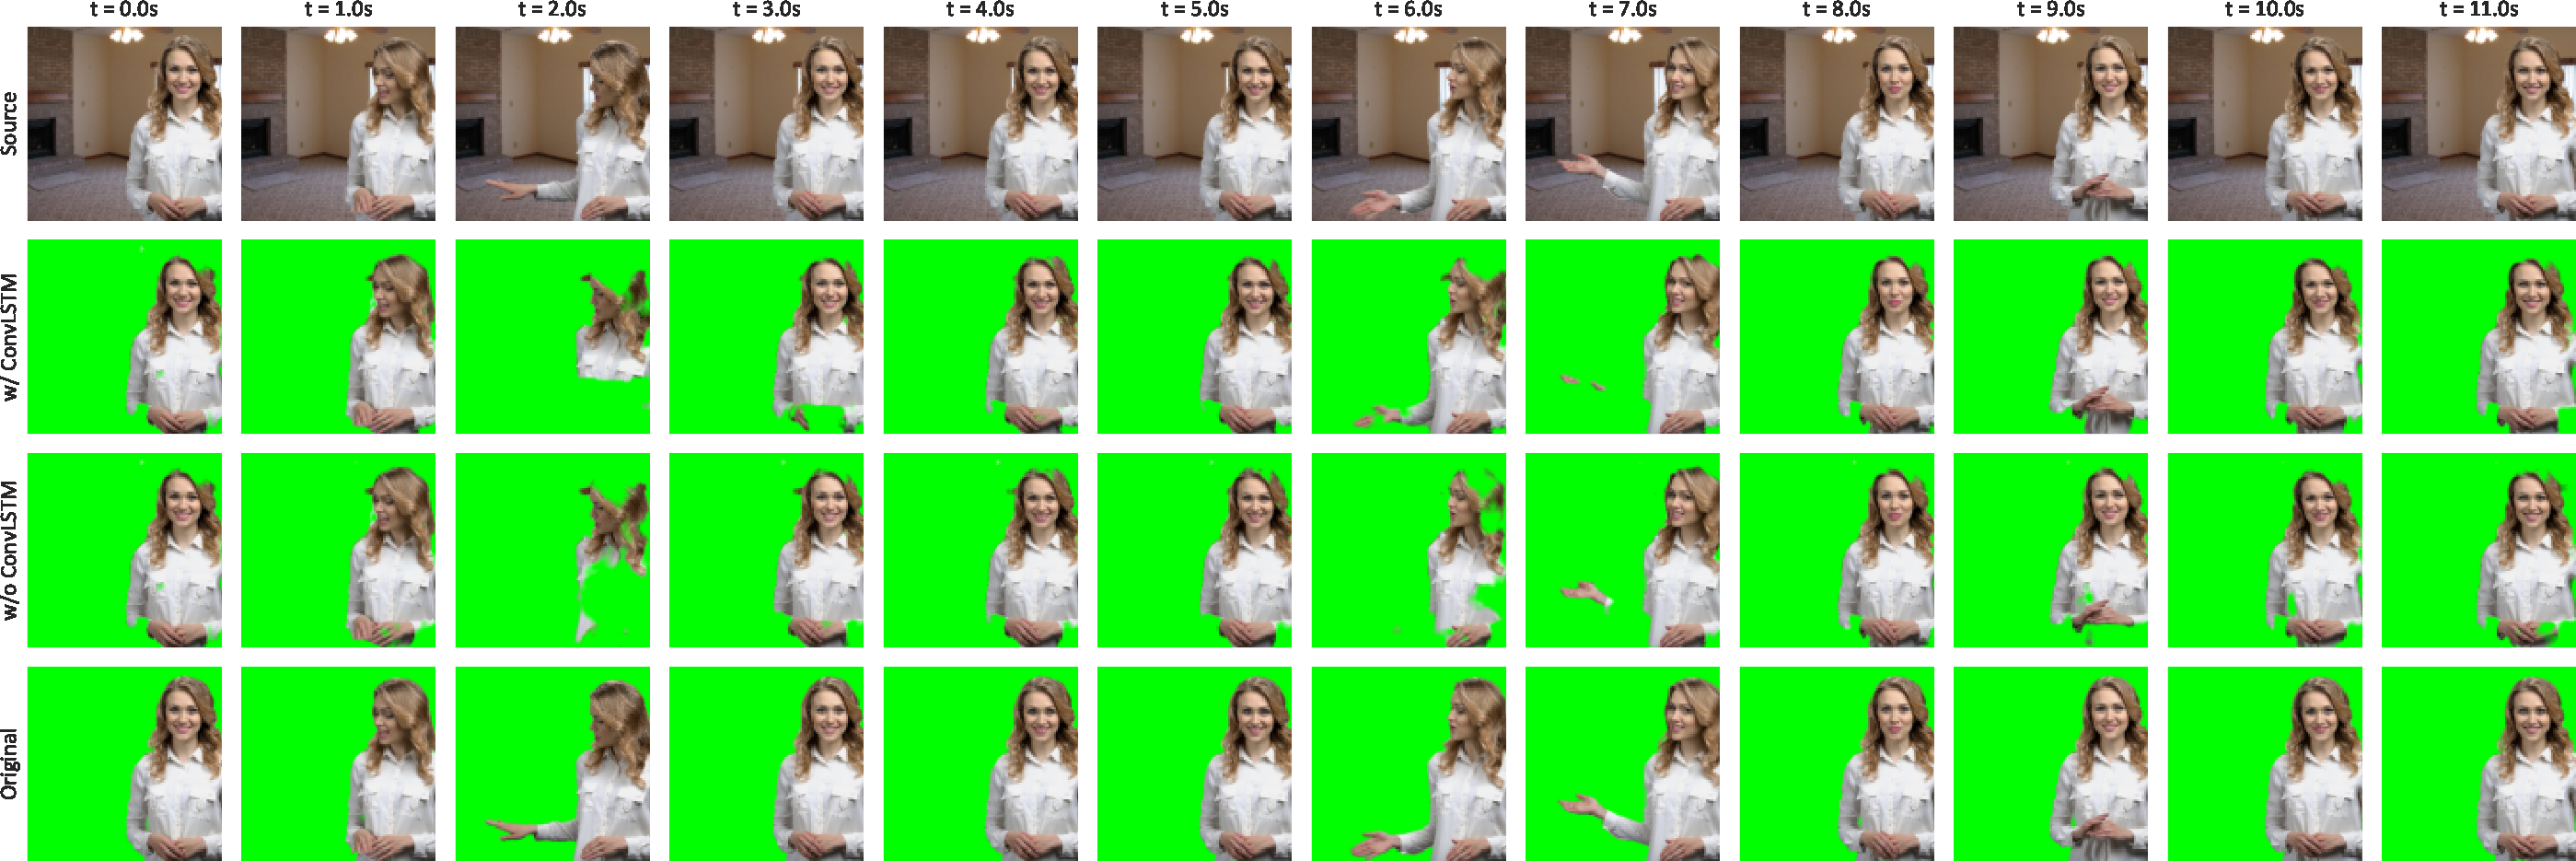
\includegraphics[width=1\textwidth]{img/visual.pdf}
    \end{center}
    \caption{Visualization of matting result at different frame across three models.}
    \label{visual}
\end{figure*}

To measure the quantitative performance between the predicted alpha matte $\alpha'$ and ground truth $\alpha^*$, we use the following four metrics proposed by \cite{Rhemann2009APM}.

\paragraph{MAD (Mean Absolute Difference)}

\begin{equation}\label{mad}
    \operatorname{MAD}(\alpha', \alpha^*)=\Vert\alpha'-\alpha^*\Vert_1
\end{equation}

\paragraph{MSE (Mean Squared Error)}

\begin{equation}\label{mse}
    \operatorname{MSE}(\alpha', \alpha^*)=\Vert\alpha'-\alpha^*\Vert_2^2
\end{equation}

\paragraph{GRAD (Spatial-Gradient Metric)}

\begin{equation}\label{grad}
    \operatorname{GRAD}(\alpha', \alpha^*)=\frac{1}{1000}\sum_i(\nabla \alpha'_i-\nabla \alpha^*_i)^q
\end{equation}

where we compute the sum of gradient difference on normalized alpha mattes.
The $\alpha'_i$ and $\alpha^*_i$ are normalized from $\alpha'$ and $\alpha^*$ respectively.
And the $\nabla$ denotes the first-order Gaussian derivative filters with variance $\sigma=1.4$. $q=2$ following \cite{linRealTimeHighResolutionBackground2020a}.
Then scale down 1000 times for better readability.

\paragraph{CONN (Connectivity)}

\begin{equation}\label{conn}
    \operatorname{CONN}(\alpha', \alpha^*)=\frac{1}{1000}\sum_i\Vert\varphi(\alpha'_i,\Omega)-\varphi(\alpha^*_i,\Omega)\Vert_1
\end{equation}

The fewer differences does not always mean better performance, connectivity of predicted alpha matte is also essential.
As shown in Equation \ref{conn}, $\varphi(\alpha_i,\Omega)$ means the connectivity for pixel $i$ in alpha matte $\alpha$ to the connected region source $\Omega$.
E.g. if $\varphi=1$, the pixel it fully connected, $\varphi=0$, the pixel is not connected at all. Instead of using power of $p$, L1 norm is used here.
Then scale down 1000 times for better readability.

\subsubsection{Implementation}

Most code are adapted from the repositories on GitHub listed in Table \ref{repository}.
The whole training process ran on a laptop with 8-core CPU at 3.80GHz with 32GB memory and an external RTX 2070 GPU.
Due to the limitation of computational power, we ran 10 epochs for each experiment and set batch size to 4 and sequence length to 8.
In this setting, the average load of GPU memory is 7.6GB out of 8GB.
The original FPS (Frame Per Second) is 30, we modified it to be 10 fps by jumping pass two frames for every frame during data augmentation.
Each sequence shares a same background and each batch contains frames from different videos, as shown in Figure \ref{batch}.

The optimizer we used is AdamW \cite{Loshchilov2017FixingWD}, which is a fixed version of Adam.
The learning rate is $[1e^{-4},5e^{-4},5e^{-4}]$ for Encoder, ASPP and Decoder respectively.

Following the best practice and trade-off between speed and accuracy, we use native PyTorch automatic mixed precision.

Because in the implementation of PyTorch code, Conv2D and ConvLSTM need different input size.
We managed to solve it by flatten the input first to $BT\times C\times H \times W$, feed through Conv2D layers, e.g. EB, then un-flatten back to $B\times T\times C\times H \times W$ for training ConvLSTM module, and flatten again for the output.

Training from scratch is difficult.
We experienced a very unstable result when training from random weights (alpha matte is all black).
So, we decided to apply transfer learning from fine-tuned pre-trained \href{https://drive.google.com/drive/folders/1cbetlrKREitIgjnIikG1HdM4x72FtgBh}{model} provided by \cite{linRealTimeHighResolutionBackground2020a}.
It is trained by both $G_{base}$ and $G_{refine}$ on the multiple datasets including completed VideoMatte240K.
For transfering training, $372$ out of $380$ modules are transferred, the rest modules are the first convolutional layer (weight + bias) and three ConvLSTM layer (3 x (weight + bias)).

Each epoch takes around 45 minutes, plus two validation which takes extra 40 minutes, hence an experiment takes around 8 hours.
The training loss is shown in Figure \ref{runs}.

\subsection{Experiment Results}

To make comparsion, we did three experiments with same settings.
With ConvLSTM is what we have proposed, Without ConvLSTM shares the same architecture but setting all the cell states and hidden state to be zeros. Original denotes the pretrained model by \cite{linRealTimeHighResolutionBackground2020a}, which needs both image and background as input.

\begin{table}[h]
    \centering
    \caption{Result across different model.}
    \label{result}
    \begin{tabular}{lcccc}
        \toprule
        {}           & MAD              & MSE              & GRAD             & CONN               \\
        \midrule
        Original     & \textbf{2.04}    & \textbf{0.94}    & \textbf{0.11}    & \textbf{102.40}    \\
        \midrule
        w/ ConvLSTM  & \underline{5.98} & \underline{3.72} & \underline{4.12} & \underline{299.99} \\
        w/o ConvLSTM & 6.53             & 4.61             & 4.93             & 327.66             \\
        \bottomrule
    \end{tabular}
\end{table}

\subsubsection{Discussion}

Due the insufficient training (less data, fewer epochs, etc.), and the lack of background information, the overall performance of our implementation is far worse than the Original.
As shown in Figure \ref{visual}, the top part of hair and the bottom part of body are mis-predicted.
But the face, neck and shoulder parts are remained as good as Original.

\subsubsection{Ablation Study}

\begin{figure}[htb]
    \begin{center}
        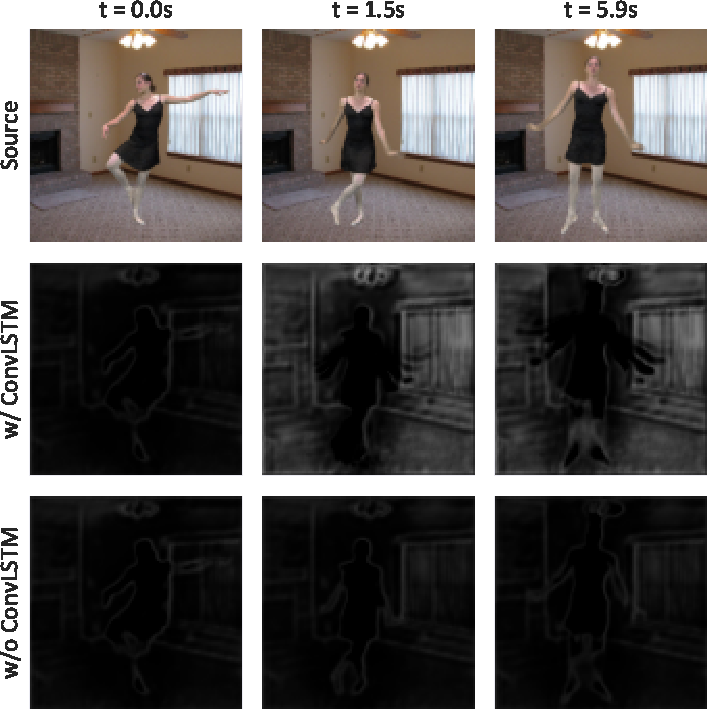
\includegraphics[width=1\linewidth]{img/ablationStudy.pdf}
    \end{center}
    \caption{Example channel of the hidden state in ConvLSTM module.}
    \label{ablationStudy}
\end{figure}

We did a ablation study on the ConvLSTM modules we added to offset the negative effects of removing the background.
As shown in Table \ref{result}, although the result of Original is much better than what we implemented, the With ConvLSTM does overperforms Without ConvLSTM.
And for qualitative comparison in Figure \ref{visual}, With ConvLSTM shows much better connectivity, clearer boundaries.
Therefore the ConvLSTM module does enhance the model for better generalization.

Then we want to know exactly how ConvLSTM helps the learning.
We record the hidden states and cell states of the last ConvLSTM module as shown in Figure \ref{ablationStudy}.
It is clear that some channels are able to learn and remember the motion of the human figure, e.g., the movements of the arms and trying to re-construct and enhance the background.
In this way, the model can obtain the unobstructed background from previous frames, therefore this method should be robust enough to run without extra background image as input.

\section{Conclusion}

Conclusion TODO

\bibliographystyle{ieee_fullname}
\bibliography{reference}

\section{Review}

\subsection{Self Reflection}

TODO

\subsection{Confidential Peer Review}

TODO

In doing this project, to the best of my judgement,
I confirm that Jiahao Zhang mainly contributed to TODO,
and his/her overall contribution is about 34\%,
Peng Zhang mainly worked on TODO,
and his/her contribution is about 33\%,
and Hang Zhang was responsible for TODO,
and his/her contribution counts about 33\% of the total project workload.

\appendix

\section{Appendix}

\begin{table}[htb]
    \centering
    \caption{Easing functions used for motion data augmentation.}
    \label{easingFunctions}
    \begin{tabular}{cccc}
        \toprule
        LinearInOut      & BackEaseIn        \\ BackEaseOut        & BackEaseInOut        \\
        BounceEaseIn     & BounceEaseOut     \\ BounceEaseInOut    & CircularEaseIn       \\
        CircularEaseOut  & CircularEaseInOut \\ CubicEaseIn        & CubicEaseOut         \\
        CubicEaseInOut   & ExponentialEaseIn \\ ExponentialEaseOut & ExponentialEaseInOut \\
        ElasticEaseIn    & ElasticEaseOut    \\ ElasticEaseInOut   & QuadEaseIn           \\
        QuadEaseOut      & QuadEaseInOut     \\ QuarticEaseIn      & QuarticEaseOut       \\
        QuarticEaseInOut & QuinticEaseIn     \\ QuinticEaseOut     & QuinticEaseInOut     \\
        SineEaseIn       & SineEaseOut       \\ SineEaseInOut \\
        \bottomrule
    \end{tabular}
\end{table}

\begin{table*}[htb]
    \centering
    \caption{GitHub repositories used for this project.}
    \label{repository}
    \begin{tabular}{ll}
        \toprule
        Repository                                                                                                                                                & Description                           \\
        \midrule
        \href{https://github.com/PeterL1n/BackgroundMattingV2}{Real-Time High-Resolution Background Matting}\cite{linRealTimeHighResolutionBackground2020a}       & Basic model and project structure     \\
        \href{https://github.com/PeterL1n/RobustVideoMatting}{Robust High-Resolution Video Matting with Temporal Guidance}\cite{linRobustHighResolutionVideo2021} & Data augmentation, loader and metrics \\
        \href{https://github.com/ndrplz/ConvLSTM_pytorch}{Convolutional LSTM Network}\cite{shiConvolutionalLSTMNetwork2015}                                       & ConvLSTM module                       \\
        \bottomrule
    \end{tabular}
\end{table*}

\begin{figure*}[htb]
    \begin{center}
        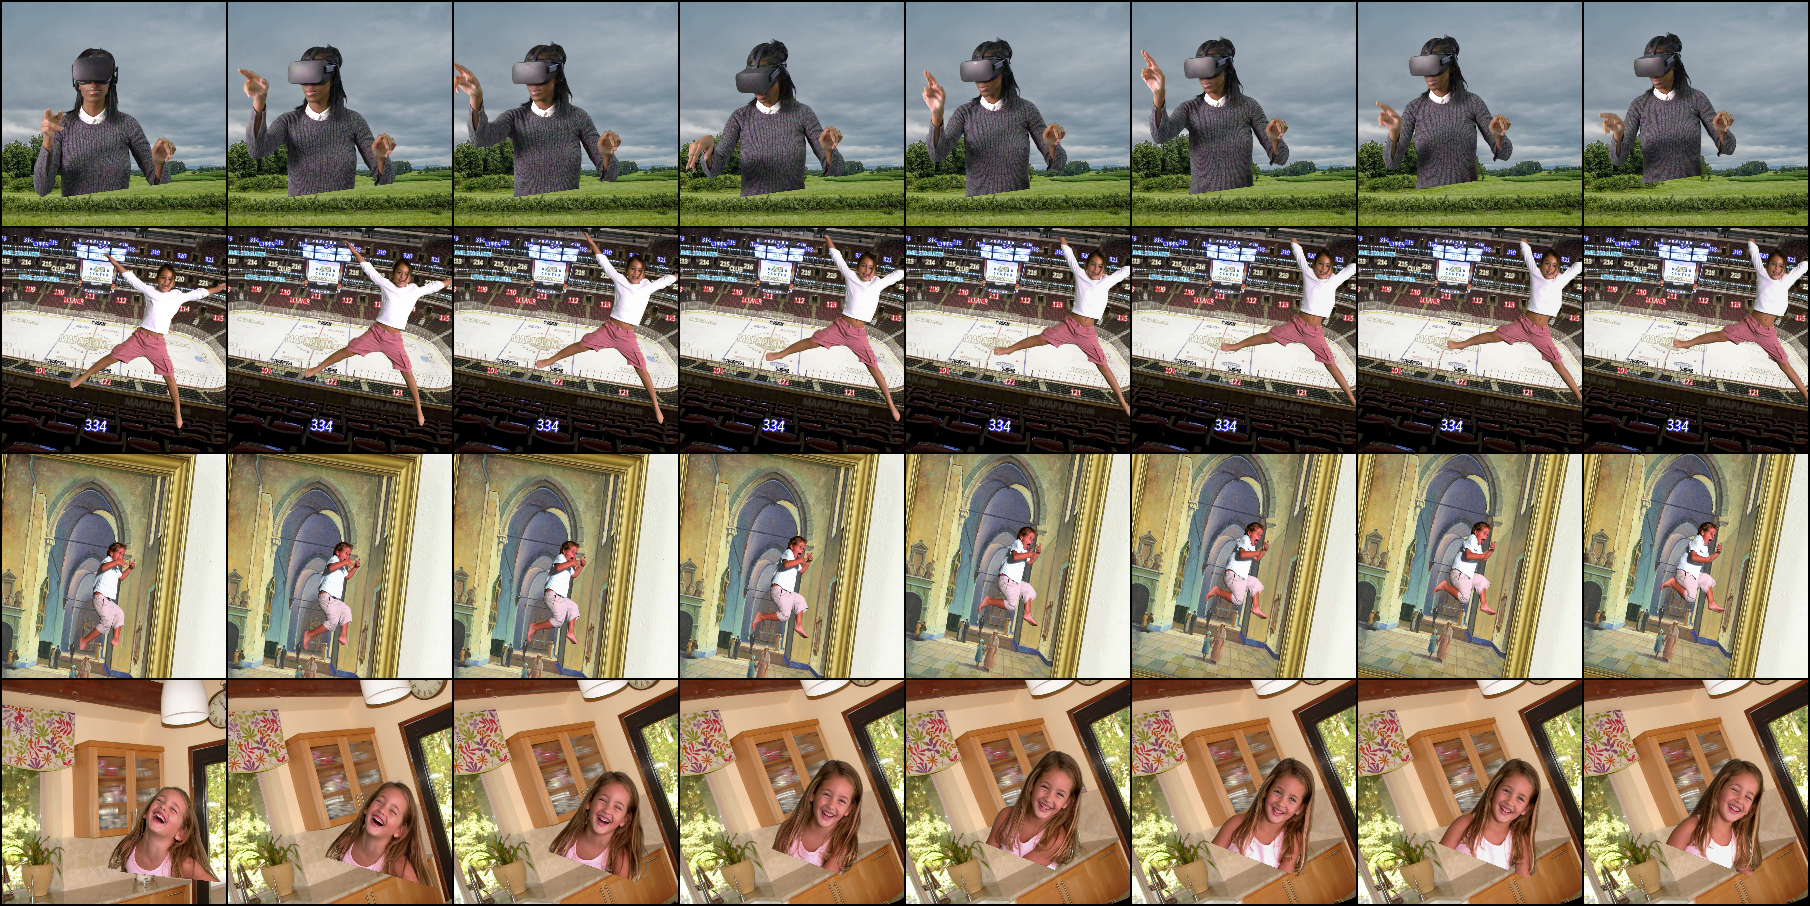
\includegraphics[width=1\textwidth]{img/batch.png}
    \end{center}
    \caption{Demonstration of a batch.}
    \label{batch}
\end{figure*}

\begin{figure*}[htb]
    \begin{center}
        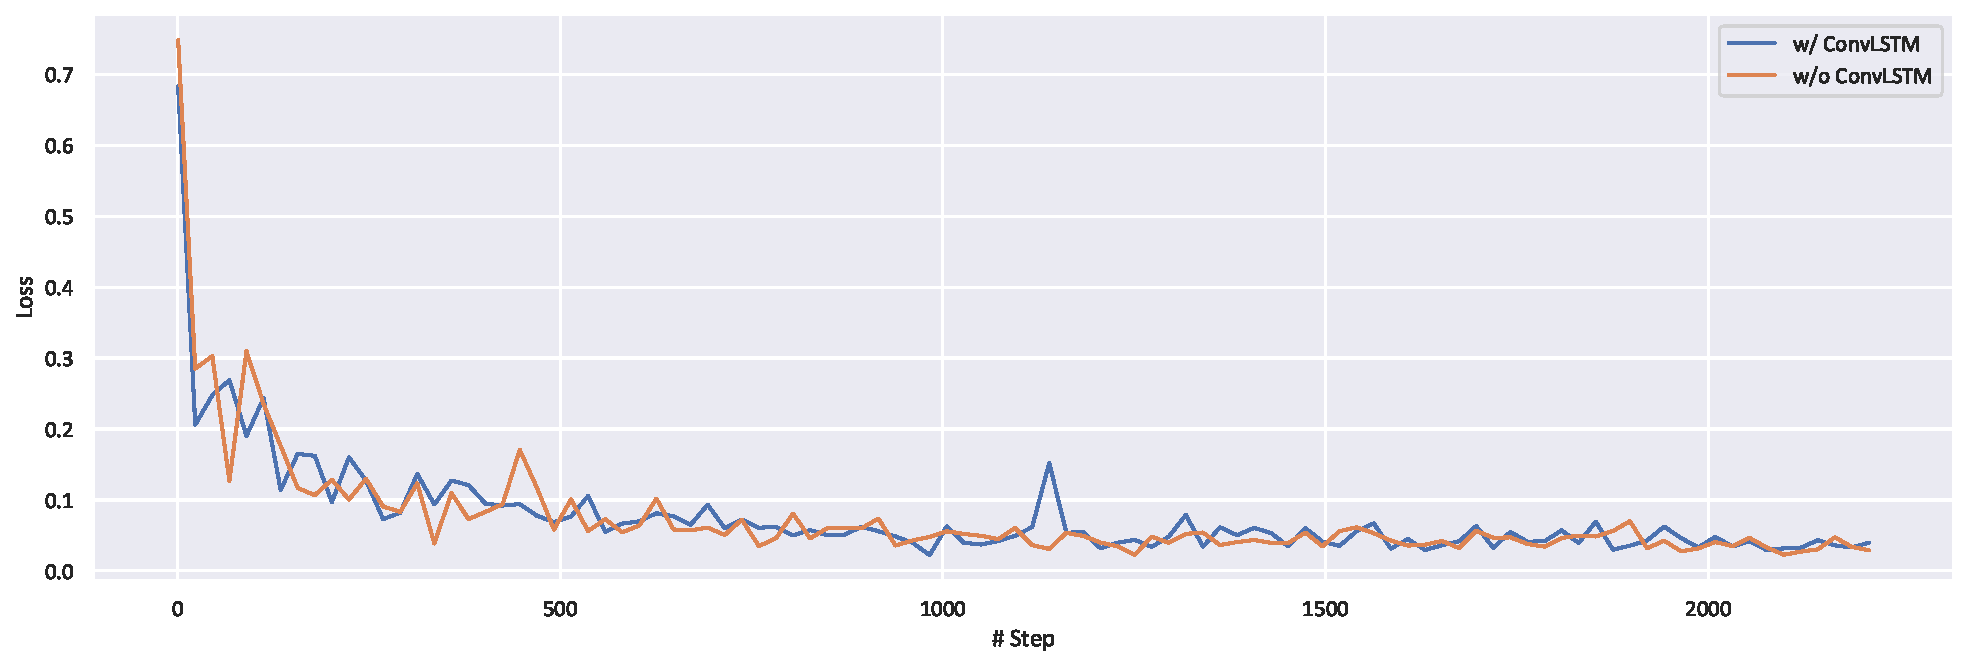
\includegraphics[width=1\textwidth]{img/runs.pdf}
    \end{center}
    \caption{Training loss.}
    \label{runs}
\end{figure*}

\end{document}
